I denne opgave skal I programmere spillet Awari, som er en variant af
Kalaha. Awari er et gammelt spil fra Afrika, som spilles af 2
spillere, med 7 pinde og 36 bønner. Pindene lægges så der dannes 14
felter ('pits' på engelsk), hvoraf 2 er hjemmefelter.  Bønnerne
fordeles ved spillet start med 3 i hvert felt pånær i
hjemmefelterne. Startopstillingen er illustreret i
Figur~\ref{fig:awari}.
\begin{figure}[h]
  \centering
  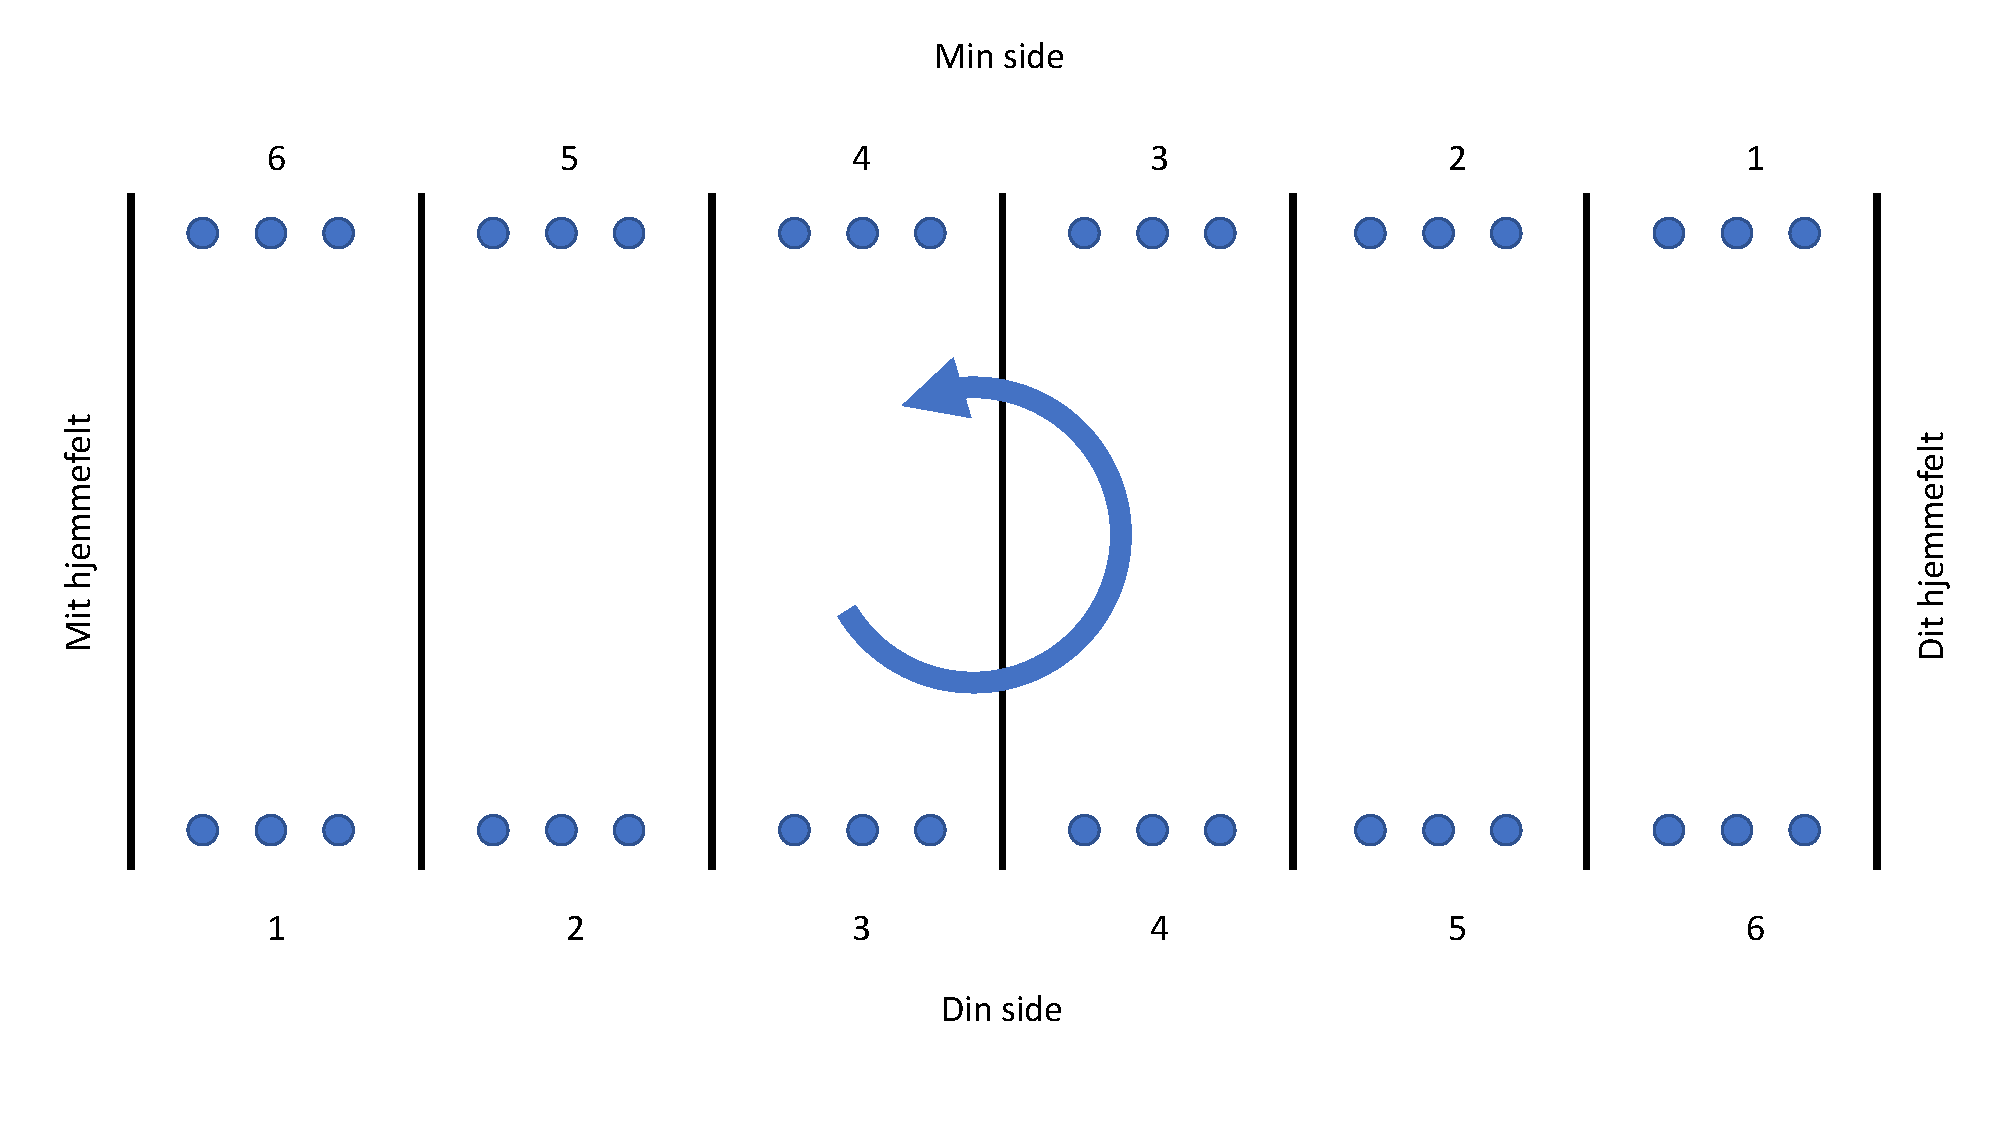
\includegraphics[width=0.75\textwidth]{awari.pdf}
  \caption{Udgangsopstillingen for spillet Awari.}
  \label{fig:awari}
\end{figure}

Spillerne skiftes til at spille en tur efter følgende regler:
\begin{itemize}
\item En tur spilles ved at spilleren tager alle bønnerne i et af
  spillerens felter 1-6 og placerer dem i de efterfølgende felter
  inkl. hjemmefelterne en ad gangen og mod uret. F.eks., kan første
  spiller vælge at tage bønnerne fra felt 4, hvorefter spilleren skal
  placere en bønne i hver af felterne 5, 6 og hjemmefeltet.
\item Hvis sidste bønne lægges i spillerens hjemmefelt, får spilleren
  en tur til.
\item Hvis sidste bønne lander i et tom felt som ikke er et hjemmefelt, og
  feltet overfor indeholder bønner, så flyttes sidste bønne til
  spillerens hjemmefelt, og alle bønnerne overfor fanges og flyttes ligså til
  hjemmefeltet.
\item Spillet er slut når en af spillerne ingen bønner har i sine
  felter 1-6, og vinderen er den spiller, som har flest bønner i sit
  hjemmefelt.
\end{itemize}
